\chapter{نصب نرم‌افزار در اوبونتو}
در این فصل به نحوهٔ نصب نرم‌افزار، یکی از مهم‌ترین کارهایی که در هر سیستم‌عامل به طور معمول انجام می‌دهیم، می‌پردازیم. برای نصب نرم‌افزار در اوبونتو دو راه وجود دارد: استفاده از رابط گرافیکی تقریباً جدید اوبونتو به نام \lr{Ubuntu Software Center} و استفاده از \lr{Apt} و رابط خط فرمان. البته نرم‌افزاری به نام \lr{Synaptic} هم وجود دارد که یک رابط گرافیکی برای \lr{Apt} ارائه می‌دهد و در همین فصل به معرفی آن می‌پردازیم.

\section[آشنایی با Center Software Ubuntu]{آشنایی با \lr{Ubuntu Software Center}}
مرکز نرم‌افزاری اوبونتو از نسخهٔ ۹/۱۰ به اوبونتو اضافه شد و هدف آن ساده‌تر شدن نصب برنامه در اوبونتو بود. تا قبل از ارائهٔ \lr{Ubuntu Software Center}، نصب نرم‌افزار در اوبونتو تنها از راه دستورات \lr{Apt} و \lr{Synaptic} ممکن بود و به همین دلیل، کاربران تازه‌کار با مشکلات زیادی روبه‌رو بودند. مرکز نرم‌افزاری اوبونتو رابط زیبایی دارد و شبیه بیش‌تر \lr{Sofware Center}های کنونی است.

\subsection[محیط Center Software Ubuntu]{محیط \lr{Ubuntu Software Center}}
آیکن \lr{Software Center} به صورت پیش‌فرض در اجراگر قرار دارد. اگر هم آن را حذف کرده‌اید، آن را جست‌وجو و اجرا کنید. پنجرهٔ اصلی مرکز نرم‌افزاری اوبونتو باز می‌شود.

\begin{center}
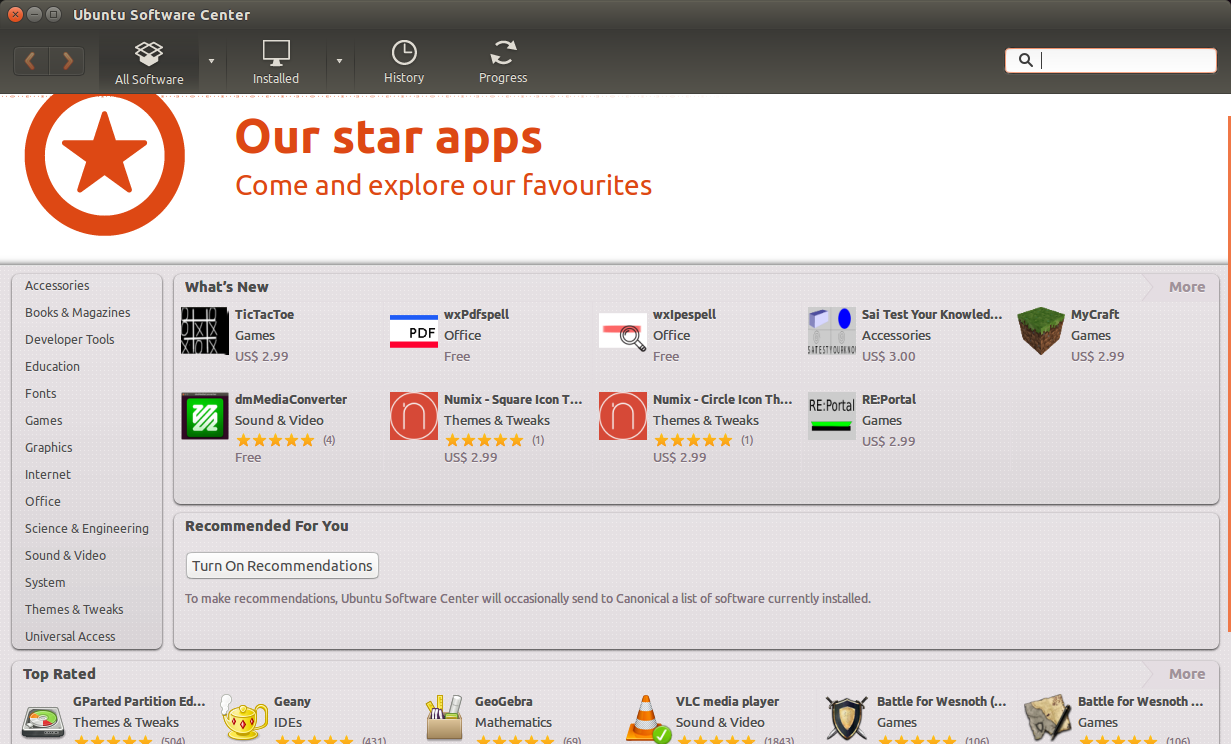
\includegraphics[scale=0.4]{pics/35.png}
\end{center}

این پنجره از بخش‌های مختلفی تشکیل شده است. در نوار بالایی، دکمه‌های جلورفتن و عقب‌رفتن، \lr{All Software} برای مشاهدهٔ همهٔ نرم‌افزارها، \lr{Installed} برای دیدن نرم‌افزارهای نصب‌شده، \lr{History} برای دیدن سوابق حذف و نصب نرم‌افزار، \lr{Progress} برای آگاهی از وضعیت دانلود و نصب نرم‌افزارهایی که دستور نصب‌شان را داده‌اید و کادر جست‌وجو وجود دارد. \lr{All Software} و \lr{Installed} دارای منوی بازشونده هستند که می‌توانید با انتخاب گزینه‌های آن نرم‌افزارهای یک مخزن مشخص را ببینید. \lr{USC} به صورت پیش‌فرض روی گزینهٔ \lr{All Software} قرار دارد.\\
در بخش اصلی، درست زیر نوار بالایی، \textbf{بنر نمایشی} وجود دارد که دارای حالتی تبلیغاتی است و نرم‌افزارهایی را به شما معرفی می‌کند. زیر بنر، بخش \textbf{نرم‌افزارهای تازه} وجود دارد و در پایین آن نیز بخش \textbf{نرم‌افزارهای پیشنهادی} را می‌بینید که البته باید آن را فعال کنید. در پایین صفحه هم برنامه‌هایی معرفی می‌شوند که بالاترین امتیاز را از کاربران دریافت کرده‌اند. در سمت چپ نیز لیست دسته‌بندی‌شدهٔ نرم‌افزارها وجود دارد که با کلیک روی هر یک از گزینه‌های آن می‌توانید نرم‌افزارهای همان بخش را مشاهده کنید.\\
نصب نرم‌افزار در \lr{USC} بسیار ساده است. تنها کافی است که نرم‌افزار مورد نظر خود را پیدا کنید و در صفحهٔ آن نرم‌افزار روی \lr{Install} کلیک کنید. گذرواژهٔ سیستم از شما پرسیده می‌شود و بعد از دانلودشدن فایل‌های مورد نیاز، برنامه نصب خواهد شد.

\section[آشنایی با Apt]{آشنایی با \lr{Apt}}
\lr{Apt} (مخفف \lr{Advanced Packaging Tool})، برنامهٔ نصب و حذف نرم‌افزارها در توزیع دبیان گنو/لینوکس است. از آن‌جایی که اوبونتو از دبیان مشتق شده است، اوبونتو نیز \lr{Apt} را به همراه دارد. نرم‌افزارهایی مثل \lr{Ubuntu Software Center} و \lr{Synaptic} هم تنها رابطی گرافیکی برای \lr{Apt} اند. پس آشنایی با \lr{Apt} می‌تواند در کنترل بیش‌تر بر سیستم به ما کمک کند.

\subsection{لیست مخازن}
برای این که \lr{Apt} کار کند، به لیست مخازن نیاز دارد. لیست مخازن شامل آدرس مکان‌هایی است که می‌توان از آن‌جا برای اوبونتو نرم‌افزار تهیه کرد. یکی از تفاوت‌های اصلی ویندوز و گنو/لینوکس نیز همین است. در اوبونتو به احتمال خیلی زیاد به هیچ‌گونه \lr{CD} و \lr{DVD}ای برای نصب نرم‌افزارها نیاز نخواهید داشت. حتا اغلب اوقات هم لازم نیست برای نصب یک نرم‌افزار به دنبال فایل نصب‌اش در اینترنت بگردید. بیش‌تر نرم‌افزارهای مورد نیاز در مخازن رسمی اوبونتو موجودند.\\
مخازن رسمی اوبونتو روی اینترنت‌اند. هرچند تمام نرم‌افزارهای مخازن اوبونتو بر روی چند \lr{DVD} هم قابل تهیه است، اما باید توجه داشت که نرم‌افزارهای مخازن همیشه در حال به‌روزآوری‌اند. پس برای استفاده از جدیدترین نسخه‌های نرم‌افزارها به اینترنت نیازمندید. البته حجم نرم‌افزارهای اوبونتو (و کلاً گنو/لینوکس‌ها)، به مراتب از ویندوز کم‌تر است. دلیل این موضوع، استفاده‌کردن نرم‌افزارهای گنو/لینوکسی از ابزارها و کتاب‌خانه‌های مشترک است.\\
\subsubsection{محل لیست مخازن}
لیست مخازن در گنو/لینوکس‌های بر پایهٔ دبیان (شامل اوبونتو)، یک فایل متنی به نام \lr{sources.list} است که در مسیر \lr{\texttt{/etc/apt/sources.list}} قرار دارد. برای ویرایش این فایل، باید فایل را در ویرایشگرهای متن باز کنید. در اوبونتو، دو ویرایشگر \lr{gedit} و \lr{Nano} وجود دارد که به ترتیب گرافیکی و متنی‌اند. کار با \lr{gedit} بسیار راحت‌تر از \lr{Nano} است، پس فایل را با \lr{gedit} باز می‌کنیم. اما ویرایش‌کردن فایل لیست مخازن نیازمند اجازهٔ ریشه است؛ در نتیجه، راحت‌ترین راه بازکردن این فایل با مجوز ریشه، استفاده از دستور \lr{\texttt{sudo gedit /etc/apt/sources.list}} است.\\
بعد از زدن دستور، پنجره‌ای مانند پنجرهٔ زیر باز می‌شود.\\
تعدادی خط را می‌بینید. اگر خطی در ابتدایش علامت \lr{\texttt{\#}} وجود داشته باشد، غیرفعال است. بقیه فعال‌اند و \lr{Apt} آن‌ها را می‌خواند.

\begin{center}
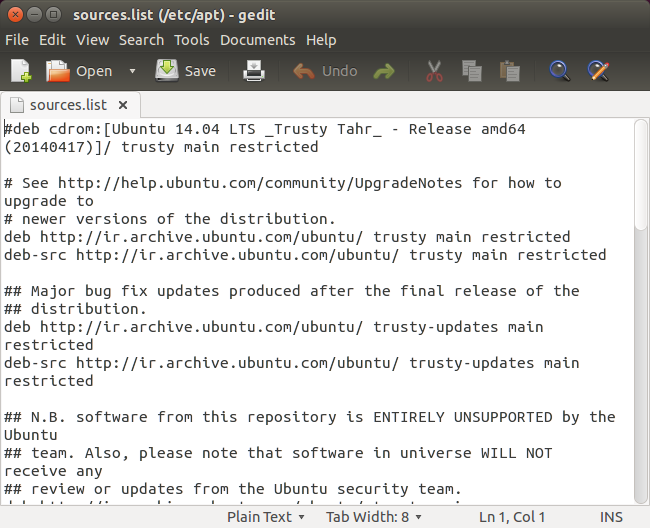
\includegraphics[scale=0.5]{pics/36.png}
\end{center}

\subsubsection{مفهوم خطوط لیست مخازن}
هر خط در این فایل شامل ۴ بخش به شکل \lr{\texttt{deb address distro component1 component2}} است. بخش اول، یعنی «\lr{\texttt{deb}}»، مشخص می‌کند که آرشیو مورد نظر دارای فایل‌های نصب با پسوند \lr{deb} است. در این بخش، به جای «\lr{\texttt{deb}}»، «\lr{\texttt{deb-src}}» هم می‌تواند قرار بگیرد که یعنی آرشیو دارای فایل‌های منبع است، نه فایل‌های نصب دبیانی.\\
در بخش دوم یا «\lr{\texttt{address}}»، باید آدرس مخزن را وارد کنید که می‌تواند آدرسی اینترنتی یا آدرسی محلی و روی کامپیوتر یا شبکهٔ خانگی‌تان باشد، اما اکثراً این یک آدرس اینترنتی است.\\
در بخش «\lr{\texttt{distro}}»، نام توزیع کنونی‌تان را وارد کنید. مثلاً برای اوبونتوی ۱۴/۰۴، باید «\lr{\texttt{trusty}} نوشته شود.\\
در آخرین قسمت هم نوع مخزن را وارد می‌کنید. اوبونتو مخازن مختلفی به نام‌های «\lr{main}»، «\lr{universe}»، «\lr{multiverse}»، «\lr{restricted}» و \ldots دارد.\\
در بخش آخر، می‌توان چندین نوع مخزن را وارد کرد. یعنی بعد از قسمت سوم، هر چه که وارد شود، مربوط به نوع مخزن خواهد بود.

\subsection[دستورهای معمول و اصلی Apt]{دستورهای معمول و اصلی \lr{Apt}}
\lr{Apt} نام یک ابزار است و اصولاً دستوری به شکل \lr{\texttt{apt}} وجود ندارد. برای استفاده از ابزار \lr{Apt}، باید از دستورهای زیرمجموعهٔ آن، مثل \lr{\texttt{apt-get}} و \lr{\texttt{apt-cache}} استفاده کرد. دستور \lr{\texttt{apt-get}}، بیش‌ترین استفاده را برای ما دارد.

\subsubsection[apt-get]{\lr{apt-get}}
همان‌گونه که گفته شد، دستور \lr{\texttt{apt-get}} مهم‌ترین دستور است. چون این دستور در بعضی فایل‌ها و پوشه‌های اصلی سیستم تغییر ایجاد می‌کند، برای استفاده از آن، باید کاربر ریشه بود (یعنی باید با \lr{\texttt{sudo}} همراه شود).\\
از این دستور برای کارهای زیر استفاده می‌شود:

\begin{description}
\item [به‌روزآوری لیست نرم‌افزارهای مخازن]: با به کار بردن دستور \lr{\texttt{sudo apt-get update}}
\item [نصب نرم‌افزار]: با دستور \lr{\texttt{sudo apt-get install software}} که به جای \lr{\texttt{software}}، باید نام نرم‌افزار مورد نظر خود را بنویسید. اگر حجم فایل‌هایی که قرار است دانلود شود زیاد باشد، پیامی مبنی بر تأیید دانلود و نصب نرم‌افزار ظاهر می‌شود که با زدن دکمهٔ \lr{Enter} تأیید می‌شود.\\
از این دستور برای نصب نسخهٔ جدید نرم‌افزار هم می‌توان استفاده کرد.
\item [حذف نرم‌افزار]: با دستور \lr{\texttt{sudo apt-get remove software}} نرم‌افزار حذف می‌شود، اما فایل‌های پیکربندی آن روی سیستم باقی می‌ماند. برای حذف نرم‌افزار همراه با حذف فایل‌های پیکربندی آن، از دستور \lr{\texttt{sudo apt-get purge software}} استفاده کنید.
\item [آپدیت‌کردن همهٔ نرم‌افزارها]: برای این کار از دستور \lr{\texttt{sudo apt-get upgrade}} استفاده کنید.
\item [آپگرید به نسخهٔ جدید اوبونتو]: این کار با آپدیت‌کردن نرم‌افزارها متفاوت است. با آپگرید، نسخهٔ اوبونتو عوض می‌شود و بعد از آپگرید، از مخازن نسخهٔ جدید اوبونتو که زودتر آپدیت می‌شوند، استفاده می‌شود. برای آپگرید از دستور \lr{\texttt{sudo apt-get dist-upgrade}} استفاده کنید.
\item [دانلود بسته‌ها]: برای دانلود بسته‌ها بدون نصب آن‌ها در پوشهٔ کنونی، از \lr{\texttt{sudo apt-get download software}} استفاده کنید.
\end{description}

\subsection[مخازن ppa]{مخازن \lr{ppa}}
مسلماً راه‌پیداکردن یک نرم‌افزار به مخازن رسمی اوبونتو کاری زمان‌بر است و نرم‌افزار باید سودمند و کارا بودن خود را ثابت کرده باشد. اما اگر بخواهید یک نرم‌افزار جدید را که به تازگی نسخه‌های اولیهٔ آن منتشر شده است، امتحان کنید چه؟\\
در اوبونتو و کلاً همهٔ گنو/لینوکس‌ها، تقریباً امکان نصب هر برنامه‌ای (خارج از مخازن) وجود دارد، اما برای نصب این برنامه‌های خارج از مخازن، باید حوصلهٔ کافی برای کامپایل‌کردن و/یا رفع وابستگی‌ها داشته باشید. آیا راه حل دیگری هم وجود دارد؟\\
خوشبختانه بله: \lr{PPA}. \lr{PPA} (مخفف \lr{Personal Package Archives}) یک منبع نرم‌افزاری برای برنامه‌نویسان است تا برنامهٔ‌شان را مستقیماً برای کاربران اوبونتو منتشر کنند. \lr{PPA} را می‌توان روی وب‌گاه دلخواه قرار داد، اما شرکت پشتیبانی‌کنندهٔ اوبونتو، کنونیکال، از چند سال پیش وب‌گاهی را به نام \href{https://launchpad.net}{\lr{Launchpad}} اختصاصاً برای میزبانی \lr{PPA} برای نرم‌افزارهای آزاد/متن‌باز راه‌اندازی کرده است.\\


\subsubsection[نحوهٔ کار با مخازن ppa]{نحوهٔ کار با مخازن \lr{ppa}}
برای پیداکردن یک \lr{ppa}، در کادر جست‌وجوی صفحهٔ اصلی لانچپد، «\lr{package ppa}» را بنویسید (به جای \lr{package} نام برنامهٔ موردنظر را تایپ کنید).\\
بعضی از برنامه‌ها چند مخزن مختلف دارند (مانند \lr{ppa}، \lr{unstable} و ...). معمولاً مخزن \lr{ppa} مناسب‌ترین مخزن است. با کلیک روی آن، صفحه‌ای مانند صفحهٔ زیر را می‌بینید.\\
\begin{center}
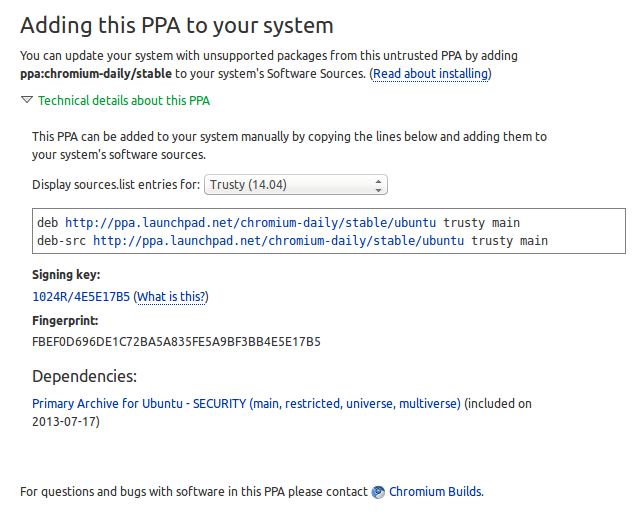
\includegraphics[scale=0.5]{pics/37.png}
\end{center}

در این صفحه اطلاعاتی در مورد آدرس \lr{ppa} نشان داده می‌شود. می‌توان \lr{ppa} را مانند مخزنی عادی به فایل \lr{\texttt{/etc/apt/sources.list}} اضافه کرد، اما در نسخه‌های اخیر اوبونتو ابزاری برای اضافه‌کردن مستقیم \lr{ppa} از راه ترمینال (یا رابط گرافیکی آن) گنجانده شده است. کافی است که دستور \lr{\texttt{sudo add-apt-repository ppa:ppa-address}} را در ترمینال وارد کنید. بعد از واردکردن دستور، کمی صبر کنید تا تأییدیهٔ افزودن مخزن ظاهر شود. برای تایید آن، کلید \lr{Enter} را فشار دهید و باز هم صبر کنید تا مخزن همراه کلید آن به مجموعهٔ مخازن سیستم‌تان افزوده شود. مدت زمان این عملیات کاملاً به سرعت و وضعیت اینترنت‌تان بستگی دارد.

\subsection[نرم‌افزار گرافیکی Synaptic]{نرم‌افزار گرافیکی \lr{Synaptic}}
در صورتی که با استفاده از \lr{Ubuntu Software Center} احساس می‌کنید روی سیستم کنترل کافی ندارید و استفاده از \lr{apt} هم برای‌تان سخت است، می‌توانید از \lr{Synaptic} استفاده کنید. \lr{Synaptic} در واقع رابطی گرافیکی برای \lr{apt} است. با استفاده از سیناپتیک می‌توانید تک‌تک نرم‌افزارها و کتاب‌خانه‌های موجود در مخازن اضافه‌شده به اوبونتوتان را مشاهده کنید.\\
\lr{Synaptic} در نسخه‌های قدیمی اوبونتو جزو نرم‌افزارهای پیش‌فرض اوبونتو بود، اما در نسخه‌های اخیر، با اضافه‌شدن \lr{Ubuntu Software Center}، سیناپتیک از نرم‌افزارهای پیش‌فرض اوبونتو حذف شد. برای همین باید آن را با استفاده از \lr{apt} یا \lr{USC} نصب کنید.

\begin{center}
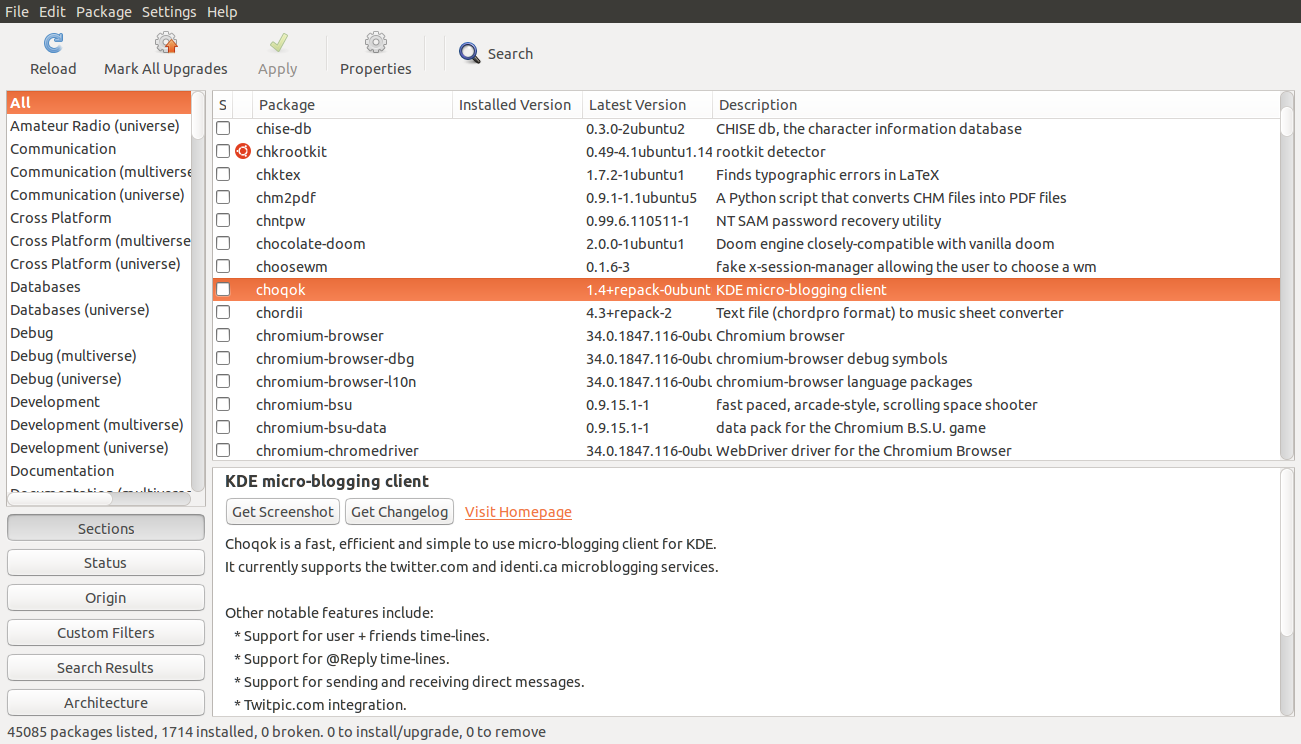
\includegraphics[scale=0.37]{pics/38.png}
\end{center}


\subsection[dpkg]{\lr{dpkg}}
\lr{dpkg} در واقع برنامهٔ اصلی حذف و نصب نرم‌افزار در دبیان است و همهٔ نرم‌افزارهایی که در این بخش معرفی شدند، برای نصب نرم‌افزار از \lr{dpkg} استفاده می‌کنند. دلیل معرفی آن در انتهای این بخش، کاربرد نسبتاً کم آن برای کاربران عادی است. تنها زمانی به استفاده از خود \lr{dpkg} نیاز پیدا می‌کنید که بخواهید فایل با پسوند \lr{.deb} یک نرم‌افزار را دستی نصب کنید.\\

\subsubsection[پارامترهای dpkg]{پارامترهای \lr{dpkg}}
\lr{dpkg} دارای پارامترهای زیادی است. در این‌جا تنها به دو تای آن اشاره می‌شود.

\begin{description}
\item[نصب]: \lr{\texttt{sudo dpkg -i package.deb}}
\item[حذف]: \lr{\texttt{sudo dpkg -r package}}
\end{description}

\subsubsection[gdebi]{\lr{gdebi}}
\lr{gdebi} یک رابط گرافیکی برای نصب بسته‌های \lr{.deb} است (البته امکان استفاده از آن در ترمینال نیز وجود دارد). مزیت استفاده از \lr{gdebi} به جای \lr{dpkg} (علاوه بر گرافیکی‌بودن آن)، دانلودکردن و نصب همهٔ وابستگی‌های نرم‌افزاری مورد نیاز است. در صورتی که نیازمندی‌های یک بستهٔ \lr{.deb} را نصب نکرده باشید و بسته را با \lr{dpkg} نصب کنید، مدیر بسته‌های سیستم آسیب می‌بیند. این وضعیت به دلیلی که گفته شد، در \lr{gdebi} وجود ندارد.\\
برای نصب \lr{gdebi} کافی است که بستهٔ \lr{gdebi} را از مخازن دریافت و نصب کنید. بعد از نصب آن، روی بستهٔ \lr{.deb} ای که می‌خواهید نصب کنید، راست‌کلیک کنید و \lr{gdebi} را انتخاب کنید.

\begin{center}
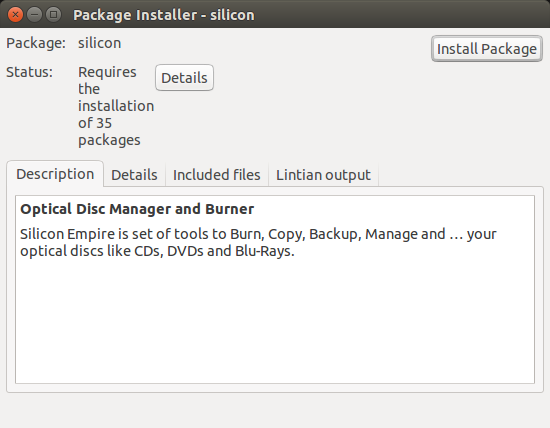
\includegraphics[scale=0.5]{pics/39.png}
\end{center}
